\documentclass{standalone}
\usepackage{tikz}
\usepackage{tikzlings-koalas}
\usetikzlibrary{calc}
\begin{document}
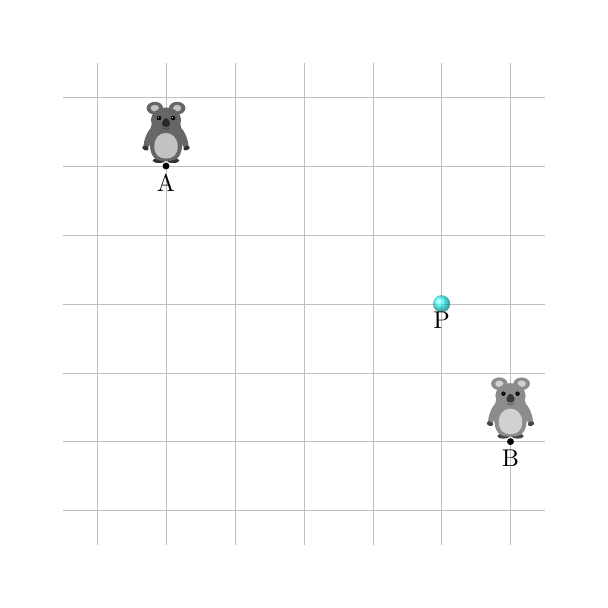
\begin{tikzpicture}[scale = 7/8, transform shape]
	\def\r{.05}
	\def\px{2}
	\def\py{0}
	\def\ax{-2}
	\def\ay{2}
	\def\bx{3}
	\def\by{-2}
	\coordinate (P) at (\px,\py);
	\coordinate (A) at (\ax,\ay);
	\coordinate (B) at (\bx,\by);
	\draw[white] (-4,-4) -- (4,4);
	\draw[step=1,gray!50!white,ultra thin] (-3.5,-3.5) grid (3.5,3.5);

    \koala[body = black!60!white,xshift = \ax cm, yshift = \ay cm, scale = .4];
	\koala[body = black!45!white,xshift = \bx cm, yshift = \by cm, scale = .4];
	\shade[ball color= cyan,opacity=0.7] (P) circle[radius=.125];
	
	\node[below] at (P) {P};
	\node[below] at (A) {A};
	\fill (A) circle ({\r});
	\node[below] at (B) {B};
	\fill (B) circle ({\r});
\end{tikzpicture}
\end{document}
